\documentclass{article}
\usepackage[utf8x]{inputenc}
\usepackage{amsmath}
\usepackage{MathUnicode}
\usepackage{upquote,textcomp}
\usepackage[a4paper,bindingoffset=0.2in,left=1in,right=1in,top=1in,bottom=1in,footskip=.25in]{geometry}

\usepackage{changepage}

\usepackage[spanish]{babel}
\usepackage{tabularx}
\usepackage{multirow}
\usepackage{graphicx}
\usepackage{listings}
\usepackage[font=scriptsize]{caption}
\usepackage[font=scriptsize]{subcaption}
\usepackage{caption}
\usepackage[yyyymmdd,hhmmss]{datetime}

\usepackage[colorlinks,urlcolor=blue]{hyperref}

\newcounter{problem}
\newcounter{solution}
\renewcommand{\theenumi}{\alph{enumi}}

\newcommand\Problem{%
  \stepcounter{problem}%
  \textbf{Problema \theproblem.}~%
  \setcounter{solution}{0}%
}

\newcommand\TheSolution{%
  \textbf{Solución:}\\%
}

\newcommand\ASolution{%
  \stepcounter{solution}%
  \textbf{Solución \thesolution:}\\%
}


\setlength{\arrayrulewidth}{1mm}
\setlength{\tabcolsep}{18pt}
\renewcommand{\arraystretch}{1.5}


\author{Pedro Valero Mejía}
\title{Ejercicios de Sistemas Informáticos II}
\parindent 0in
\parskip 1em

\begin{document}

\maketitle
%%%%%%%%%%%%%%%%%%%%%%%%%%%%%%%%%%%%%%%%%%%%%%%%%%%%%%%%%%%%%%%%%%%%%%%%%% PROBLEMA 1
\Problem
Los mensajes llegan a un servidor de descifrado de manera poissoniana con un ritmo medio de llegada de 360 mensajes por minuto. Los tiempos de descifrado son proporcionales a la longitud de los mensajes, los cuales se distribuyen aproximadamente de forma exponencial, con una longitud media de 1500 bytes. La velocidad del servidor de descifrado es de 10Kbyte/s. ¿Cuál es el tiempo medio de espera de respuesta por mensaje? ¿Cuál es el número medio de mensajes en el sistema de descifrado?

\TheSolution

El número de mensajes por unidad de tiempo es la tasa de llegadas, que deberemos escribir en unidades del Sistema Internacional:
\[λ = 360 min^{-1}=6 s^{-1}\]

Por otro lado tenemos que si la longitud del mensaje es una variable aleatoria que sigue una distribución exponencial y el tiempo de procesamiento es proporcional a la longitud, el tiempo de servicio será una variable aleatoria exponencial de media:
\[T_s = \frac{1500 bytes}{10000 bytes/s} = \boxed{0.15s}\]

A partir de aquí podemos calcular la tasa de servicio:
\[μ = \frac{1}{T_s} = 6.66 s^{-1}\]

Se trata de un sistema M/M/1 de modo que podemos calcular el número medio de mensajes en el sistema a partir, únicamente, del factor de utilización según la fórmula:
\[L=\frac{ρ}{1-ρ}=\frac{λ/μ}{1-λ/μ}=\frac{λ/μ}{(μ-λ)/μ}=\frac{λ}{μ-λ}=\boxed{9.09}\]


%%%%%%%%%%%%%%%%%%%%%%%%%%%%%%%%%%%%%%%%%%%%%%%%%%%%%%%%%%%%%%%%%%%%%%%%%% PROBLEMA 2

\Problem
Se tiene un servidor en Internet que recibe un tráfico de Poisson a un ritmo medio P peticiones/s. El tiempo que tarda en atender una petición se encuentra distribuido exponencialmente, siendo capaz de procesar S peticiones/s.

Debido al éxito del servidor, a los quince días de su aparición en Internet su tráfico se ha multiplicado por un factor K. Para resolver el problema, se cambia de ordenador, solicitando uno de potencia K veces superior al actual.

Calcular el nuevo número medio de clientes en el sistema servidor, y el nuevo tiempo de permanencia en el sistema tras la ampliación del servidor en función de los valores anteriores al cambio.

\newpage
\TheSolution

Tras el éxito del servidor pasamos a tener una tasa de llegadas:
\[λ = K \cdot P\]

Al cambiar la potencia del ordenador multiplicándola por $K$ estamos reduciendo el tiempo de servicio según ese mismo factor y multiplicando la tasa de servicio por $K$:
\[μ = S \cdot K\]

Se trata de un sistema M/M/1 donde el número de clientes en el sistema sólo depende del factor de utilización del mismo que, en este caso, no ha cambiado.

Por tanto seguimos teniendo el mismo número medio de clientes en el sistema que antes de producirse los cambios.

Para calcular el nuevo tiempo de permanencia nos apoyamos en el Teorema de Little que nos permite escribir
\[W = \frac{L}{λ}\]
puesto que $L$ no ha cambiado y λ se ha hecho $K$ veces mayor, el tiempo medio de permanencia en el sistema se ha reducido en un factor de $K$.

%%%%%%%%%%%%%%%%%%%%%%%%%%%%%%%%%%%%%%%%%%%%%%%%%%%%%%%%%%%%%%%%%%%%%%%%%% PROBLEMA 3

\Problem
Se desea diseñar un servidor para satisfacer un tráfico de Poisson con un tiempo medio entre peticiones de 10 s. El servicio a proporcionar tiene una duración distribuida exponencialmente con media de 16 s. Calcular:
\begin{enumerate}
\item El número mínimo de servidores para satisfacer el tráfico requerido.
\item Con dicho número de servidores, el tiempo medio de espera en cola por petición.
\item El tiempo medio de espera en cola, en caso de independizar cada servidores, asignándole una cola de espera a cada uno de ellos, y repartiendo el tráfico entre ellos de modo aleatorio para que cada uno reciba la mitad del total.
\end{enumerate}

\TheSolution

\begin{enumerate}
\item

Si nos llega una petición cada 10 segundos, tenemos una tasa de llegadas de
\[λ = 0.1 s^{-1}\]

Dado que el tiempo medio de servicio es de 16s y tenemos $c$ servidores, la tasa de servicio es:
\[μ=\frac{0.0625}{c}\]

Si queremos que el sistema no colapse, necesitamos que el factor de utilización sea menor que 1, es decir:
\[ρ = \frac{λ}{cμ}<1 \implies λ < cμ \implies c>1.6\]
necesitamos $\boxed{2}$ servidores para satisfacer el tráfico requerido
\item

Para este ejercicio nos apoyamos fuertemente en el formulario. Nos encontramos ante un sistema M/M/2 y para calcular el tiempo de espera en cola debemos calcular el número de clientes en el sistema con ayuda de las fórmulas. Una vez obtenido este valor aplicamos el Teorema de Little para calcular el tiempo medio de estancia en el sistema y le restamos el tiempo medio de servicio.

Vamos a ello:

\[ρ = \frac{λ}{2\cdot μ}=0.8\]

\[p_0 = \left[ \sum_{n=0}^{c-1}\frac{(λ/μ)^n}{n!}+\frac{(λ/μ)^c}{c!(1-ρ)}\right]^{-1}=\left[1+1.6+\frac{2.56}{0.4}\right]^{-1}=(9)^{-1}=0.11\]

\[p_2=p_0\frac{c^c}{c!}\left( \frac{λ}{cμ}\right)^n=0.11\cdot 2 \cdot 0.64 = 0.14\]
\[P_q=\frac{p_c}{1-ρ}=0.71\]

Finalmente
\[L=\frac{P_q ρ}{1-ρ}+cρ=4.44\]

Aplicando Little nos queda
\[W = \frac{L}{λ}=44.4\]

Puesto que el tiempo de servicio es de 8s, el tiempo medio de espera en cola asciende a
\[W-T_s=\boxed{36.4s}\]
\item

Este caso es equivalente al ejercicio anterior con $K=0.5$ por lo que tenemos
\[W_n =\frac{W_o}{K}=88.8s\]

lo que implica
\[W-T_s = \boxed{56.8s}\]
\end{enumerate}

%%%%%%%%%%%%%%%%%%%%%%%%%%%%%%%%%%%%%%%%%%%%%%%%%%%%%%%%%%%%%%%%%%%%%%%%%% PROBLEMA 4

\Problem
Se quiere diseñar un servidor de emisión de certificados en Internet para que sea capaz de atender una media de 10 peticiones por segundo con un tiempo medio de respuesta de 0.1s. Sabiendo que el programa de generación del certificado es siempre el mismo, independientemente del cliente, y requiere la ejecución de 10.000 instrucciones de código máquina, calcular la potencia de ordenador (en MIPS) necesaria para su ejecución,
suponiendo despreciable cualquier otra carga en el mismo.

\TheSolution

Queremos ejecutar 10.000 instrucciones de código en 0.1s deberemos tener una potencia de \boxed{0.1 MIPS}


%%%%%%%%%%%%%%%%%%%%%%%%%%%%%%%%%%%%%%%%%%%%%%%%%%%%%%%%%%%%%%%%%%%%%%%%%% PROBLEMA 5

\Problem
Una fracción p del tráfico de salida procedente de un servidor con tiempo de servicio distribuido exponencialmente con media Ts se realimenta a su entrada. El tráfico nuevo llega al servidor con un ritmo medio R. Calcular el factor de utilización del servidor y el tiempo medio de estancia en el
sistema.

\TheSolution

Empezamos calculando la tasa de llegadas:
\[λ = R + pλ \implies λ = \frac{R}{1-p}\]

La taasa de servicio es
\[μ= \frac{1}{T_s}\]

Así el factor de utilización sería
\[ρ=\frac{λ}{μ}=\boxed{\frac{R \cdot T_s}{1-p}}\]

Sabiendo que es un sistema M/M/1 podemos calcular el número medio de clientes en el sistema como:
\[L = \frac{ρ}{1-ρ}=\frac{R\cdot T_s}{1-p-R\cdot T_s}\]

Aplicando ahora el Teorema de Little podemos calcular el tiempo medio de estancia en el servidor como:
\[W = \frac{L}{λ}=\boxed{\frac{T_s}{(1-p-R\cdot T_s)(1-p)}}\]

%%%%%%%%%%%%%%%%%%%%%%%%%%%%%%%%%%%%%%%%%%%%%%%%%%%%%%%%%%%%%%%%%%%%%%%%%% PROBLEMA 6

\Problem
En una determinada red de área local se dispone de un servidor de comunicaciones, que actúa como encaminador de mensajes de aplicación entre la dicha red y una red remota, a la que se encuentra conectado a través de una línea dedicada de velocidad $2\cdot 10^6$ bps.

A la red de área local hay conectados un número muy grande de terminales clientes, que envían mensajes cuyo tamaño se encuentra distribuido exponencialmente con un valor medio de 1 KByte.

Se puede considerar que los mensajes llegan al servidor siguiendo un ritmo de Poisson. Se pide:
\begin{enumerate}
\item Si el servidor de comunicaciones recibe un promedio de 180 peticiones/s, calcular tiempo medio que transcurre desde que un mensaje es recibido en el servidor hasta que llega al punto destino.
\item Calcular el número máximo de peticiones por segundo que se estarán procesando si se sabe que el tamaño medio de memoria que ocupa la cola de mensajes en espera de ser procesados es de 10 KBytes.
\end{enumerate}

\TheSolution

En este ejercicio el tiempo de procesamiento de mensaje por parte del servidor es el tiempo que tarda dicho servidor en enviar el mensaje a través del enlace descrito.

\begin{enumerate}
\item
Tenemos una tasa de peticiones
\[λ = 180 s^{-1}\]

Sabiendo el tamaño medio de los mensajes y la capacidad de transmisión de la línea dedicada, podemos calcular el tiempo de servicio
\[T_s = \text{tamaño}/\text{velocidad} = 0.0041s\]

lo que nos da una tasa de servicio de
\[μ=\frac{1}{T_s}=244.14 s^{-1}\]

A partir de aquí podemos calcular el factor de utilización del sistema
\[ρ = \frac{λ}{μ}=0.74\]

y, puesto que estamos ante un sistema M/M/1 podemos calcular el número medio de clientes en el sistema como
\[L = \frac{ρ}{1-ρ}=2.85\]
y a partir del Teorema de Little calculamos el tiempo medio de estancia en el sistema, que es el dato pedido
\[W= \frac{L}{λ}= \boxed{0.016s}\]

\item

Ahora nos encontraríamos ante un sistema M/M/1/K siendo $K$ el número máximo de clientes en el sistema que se calcula como el número máximo de clientes en cola +1 (el que se está procesando).

Puesto que conocemos el tamaño de la cola y el tamaño de los mensajes, podemos calcular $K=10$ mensajes. Es decir, tenemos un sistema M/M/1/10 y nos piden calcular $L$, el número máximo de clientes en el sistema.

Los valores de λ y μ calculados en el apartado anterior siguen siendo válidos, pues no han cambiado las condiciones de llegada y procesamiento de mensajes.

Procedemos pues a calcular $L$:
\[L = \frac{λ/μ}{1-λ/μ}\frac{1-(K+1)(λ/μ)^K+K(λ/μ)^{K+1}}{1-(λ/μ)^{K+1}}=\frac{λ/μ}{1-λ/μ}\frac{1-(3)(λ/μ)^2+2(λ/μ)^{3}}{1-(λ/μ)^{3}}=\]
\[=\frac{0.74}{0.26}\frac{0.17}{0.6}=\boxed{0.81}\]

\end{enumerate}
%%%%%%%%%%%%%%%%%%%%%%%%%%%%%%%%%%%%%%%%%%%%%%%%%%%%%%%%%%%%%%%%%%%%%%%%%% PROBLEMA 7

\Problem
Deseamos instalar un servidor de envío de mensajes ("busca") a una serie de abonados. El número de abonados, que suponemos muy grande, envía mensajes a nuestro servidor, desde donde se envían a su destino mediante un sistema de transmisión por radio. Los mensajes llegan según un proceso de Poisson con una tasa de llegadas L. El tiempo de servicio (total del proceso y envío del mensaje) se puede considerar distribuido exponencialmente con valor medio S. El esquema de bloques del servicio es el siguiente:

\begin{center}
  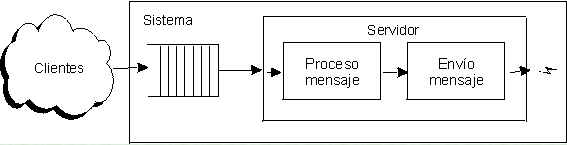
\includegraphics[keepaspectratio=true,width=\linewidth]{img/ej7.png}
  \captionof{figure}{Consola de Glassfish}
\end{center}


\begin{enumerate}
\item Calcular el tiempo medio que transcurre desde que un mensaje llega al sistema hasta que es servido a su destino.
\item La tarifa del servicio es de P Euros por mensaje transmitido, pero se proporciona un descuento de D Euros por cada segundo que el mensaje tarde en llegar a su destino. Calcular los ingresos medios esperados por mensaje transmitido.
\item Calcular a partir de qué tasa de peticiones el tiempo de espera será tal que el mensaje se deba transmitir gratuitamente (se supone que nunca se aplica un descuento mayor que el coste de transmisión del mensaje).

\end{enumerate}

\TheSolution

%%%%%%%%%%%%%%%%%%%%%%%%%%%%%%%%%%%%%%%%%%%%%%%%%%%%%%%%%%%%%%%%%%%%%%%%%% PROBLEMA 8

\Problem
Una red de una entidad financiera consta de una serie de terminales remotos, en número que podemos considerar muy grande, conectados mediante líneas telefónicas alquiladas full duplex a un multiplexor de terminales. Dicho multiplexor entrega los mensajes recibidos a un servidor, que ejecuta los programas transaccionales necesarios para atender al mensaje recibido, y devuelve los resultados al cliente a través del mismo multiplexor. El esquema de bloques del servicio es el siguiente:

\begin{center}
  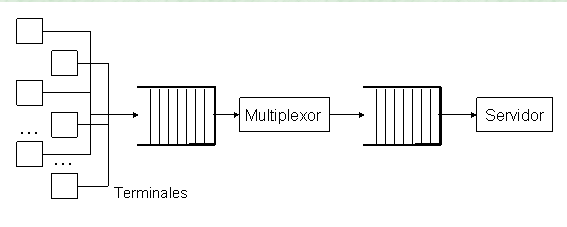
\includegraphics[keepaspectratio=true,width=\linewidth]{img/ej8.png}
  \captionof{figure}{Consola de Glassfish}
\end{center}

Los mensajes de las oficinas llegan al multiplexor según un proceso de Poisson con una tasa de llegadas total de 3 s -1 (es decir, incluyendo las peticiones de todos los servidores) y su longitud media es de 1 Kbyte. El tiempo de servicio del multiplexorpor mensaje (total del proceso y envío del mensaje) se puede considerar distribuido exponencialmente con valor medio 250 ms.

\begin{enumerate}
\item Calcular la ocupación media en memoria de la cola de mensajes en espera de servicio del multiplexor
\item Calcular la tasa de llegadas al servidor.
\item Los mensajes que llegan al servidor son de tres tipos básicos. El tiempo de proceso en el servidor depende del tipo de mensaje recibido, de acuerdo a la siguiente tabla:

\begin{center}
\begin{tabular}{| c | c | c |}
\hline
  \textbf{Identificador mensaje} & 	\textbf{Probabilidad} & \textbf{Tiempo de proceso)}\\
\hline
0	& 0.5	& 0.1 \\
1	& 0.3	& 0.2 \\
2	& 0.2	& 0.4 \\
\hline
\end{tabular}
\end{center}

Estos tiempos incluyen lo que tarda el mensaje de respuesta en llegar al terminal remoto. Esta transmisión del mensaje de respuesta se supone que no afecta al tiempo de proceso del multiplexor ni a la comunicación por la línea que lo une con el terminal.

\item Calcular el tiempo medio de estancia en el servidor de las solicitudes.


\end{enumerate}

\TheSolution

%%%%%%%%%%%%%%%%%%%%%%%%%%%%%%%%%%%%%%%%%%%%%%%%%%%%%%%%%%%%%%%%%%%%%%%%%% PROBLEMA 9

\Problem
El servidor de fecha y hora de una red resuelve cada petición en un tiempo que se puede suponer distribuido exponencialmente con media 100 ms. La red se compone de un número muy grande de clientes que realizan peticiones, cuya llegada al servidor se considera que sigue un proceso de Poisson.
\begin{enumerate}
\item Calcular el número máximo de peticiones por segundo que se podrán satisfacer para obtener un tiempo medio de respuesta del servidor menor o igual que 1 s.
\item Calcular el tiempo medio de servicio necesario para poder satisfacer el doble de peticiones reduciendo el tiempo de respuesta a la mitad.

\end{enumerate}

\TheSolution

%%%%%%%%%%%%%%%%%%%%%%%%%%%%%%%%%%%%%%%%%%%%%%%%%%%%%%%%%%%%%%%%%%%%%%%%%% PROBLEMA

\Problem



\TheSolution

%%%%%%%%%%%%%%%%%%%%%%%%%%%%%%%%%%%%%%%%%%%%%%%%%%%%%%%%%%%%%%%%%%%%%%%%%% PROBLEMA

\Problem


\TheSolution
\end{document}